\documentclass[11pt]{article}

% ==== Paquetes ====
\usepackage[utf8]{inputenc}
\usepackage[spanish]{babel}
\usepackage{amsmath, amssymb, amsfonts, siunitx}
\usepackage{graphicx}
\usepackage{float}
\usepackage{listings} % Para código
\usepackage{pdfpages}
\usepackage{xcolor}
\usepackage{hyperref}
\usepackage{caption}
\usepackage{subcaption}
\usepackage{geometry}
\usepackage{tikz}

\geometry{margin=2.5cm}

% ==== Configuración de listings (para código) ====
\lstset{
  basicstyle=\ttfamily\small,
  numbers=left,
  numberstyle=\tiny,
  stepnumber=1,
  numbersep=5pt,
  backgroundcolor=\color{gray!10},
  frame=single,
  tabsize=2,
  breaklines=true,
  showstringspaces=false,
  keywordstyle=\color{blue},
  commentstyle=\color{green!50!black},
  stringstyle=\color{red!70!black},
  literate={á}{{\'a}}1 {é}{{\'e}}1 {í}{{\'i}}1
           {ó}{{\'o}}1 {ú}{{\'u}}1 {ñ}{{\~n}}1
           {Á}{{\'A}}1 {É}{{\'E}}1 {Í}{{\'I}}1
           {Ó}{{\'O}}1 {Ú}{{\'U}}1 {Ñ}{{\~N}}1
}

% ==== Datos de la tarea ====
\title{IEE3584 - Procesamiento Avanzado de Señales \\
Tarea 3}
\author{Nicolás Seguel}
\date{Agosto 2025}

\begin{document}

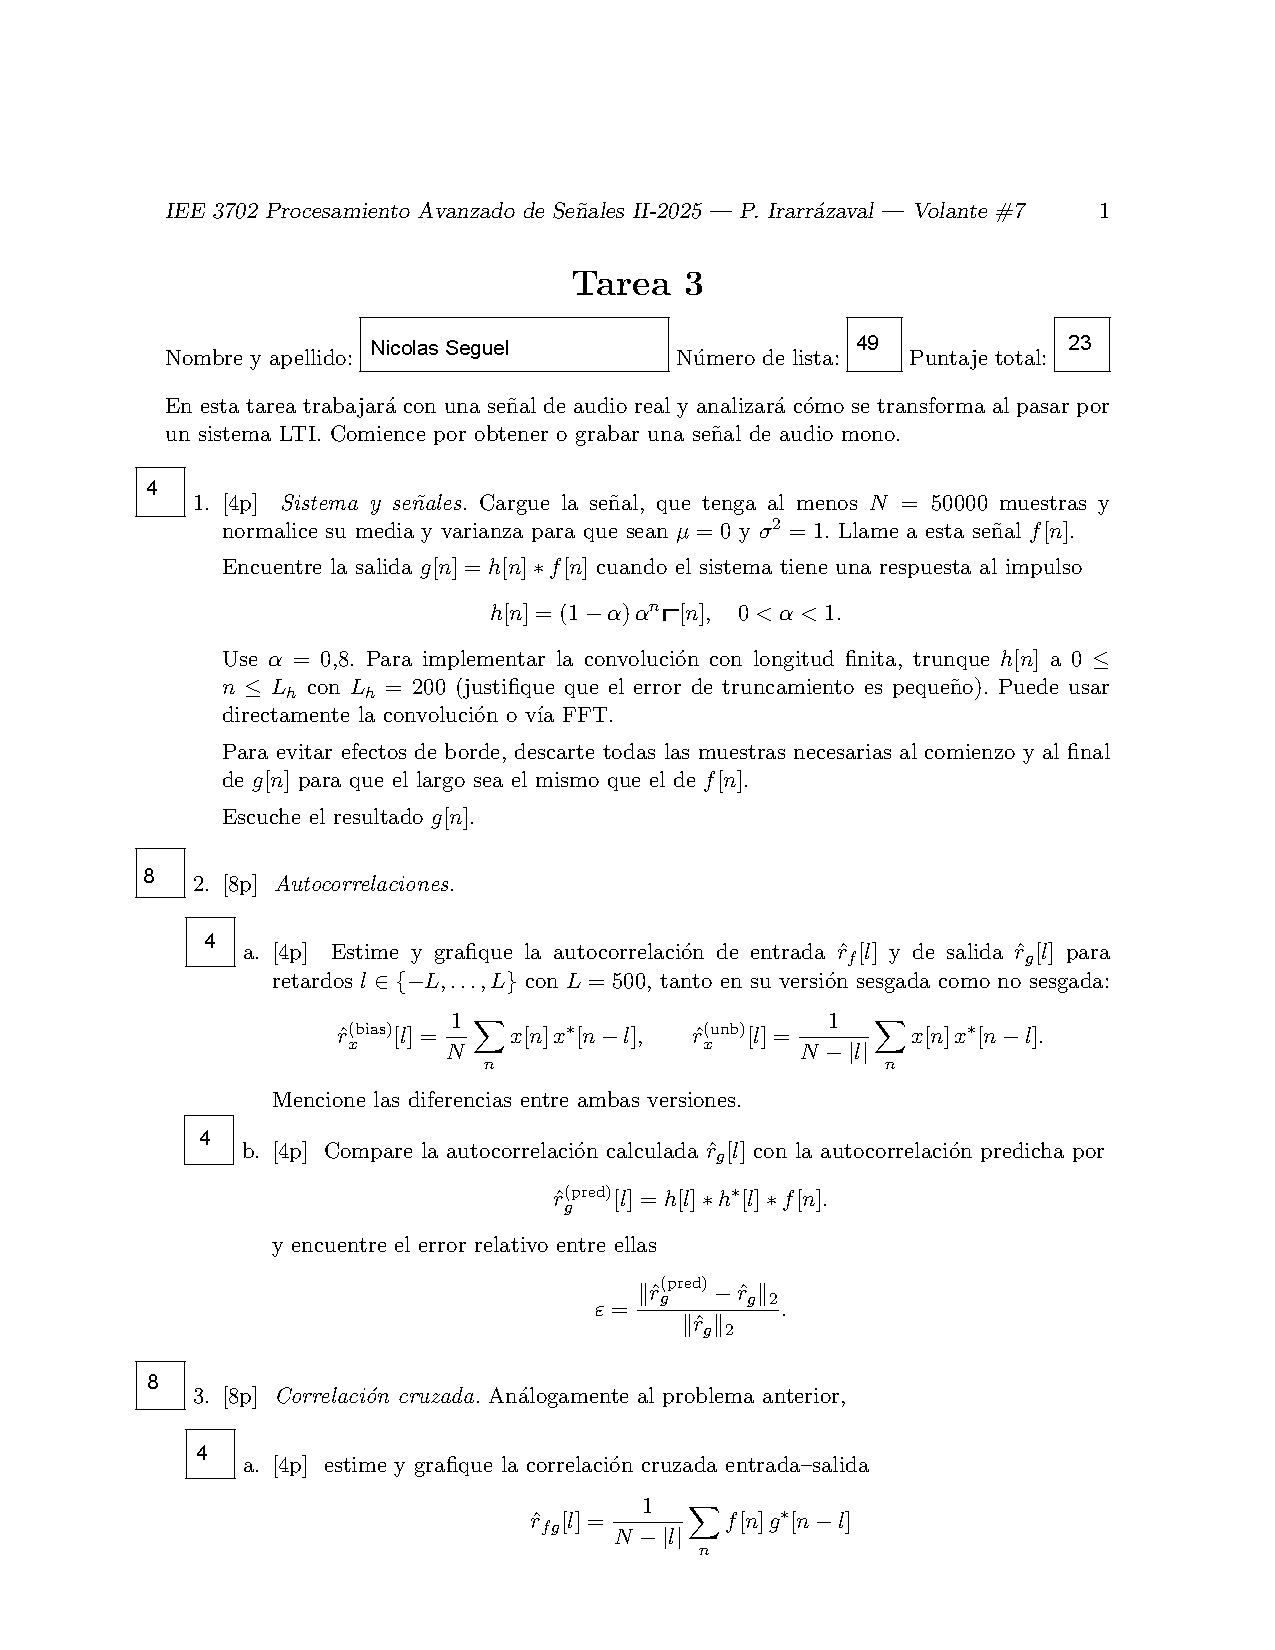
\includepdf[pages=-]{07.tarea03.pdf}
\maketitle

% ==== Problema 1 ====
\section*{Problema 1}

Se carga el archivo de audio \texttt{audio.wav}. Luego se normaliza la señal y se convoluciona con \texttt{h[n]}. Como la señal exponencial decae rápidamente, se utiliza un filtro de longitud $L_h = 200$, donde el valor de $h[n]$ se vuelve despreciable, por lo que es una buena aproximación. Finalmente, se guarda la señal resultante en \texttt{output.wav}.

\lstinputlisting[language=Python, caption={Código para el Problema 1}]{src/p1.py}

% ==== Problema 2 ====
\section*{Problema 2}

Se estiman las autocorrelaciones sesgada y no sesgada para las señales de entrada y salida, con retardos $l \in \{-500, \dots, 500\}$. Además, se compara la autocorrelación estimada de salida $\hat{r}_g[l]$ con la predicha, y se obtiene un error relativo de $0.11$.

\lstinputlisting[language=Python, caption={Código para el Problema 2}]{src/p2.py}

\begin{figure}[H]
  \centering
  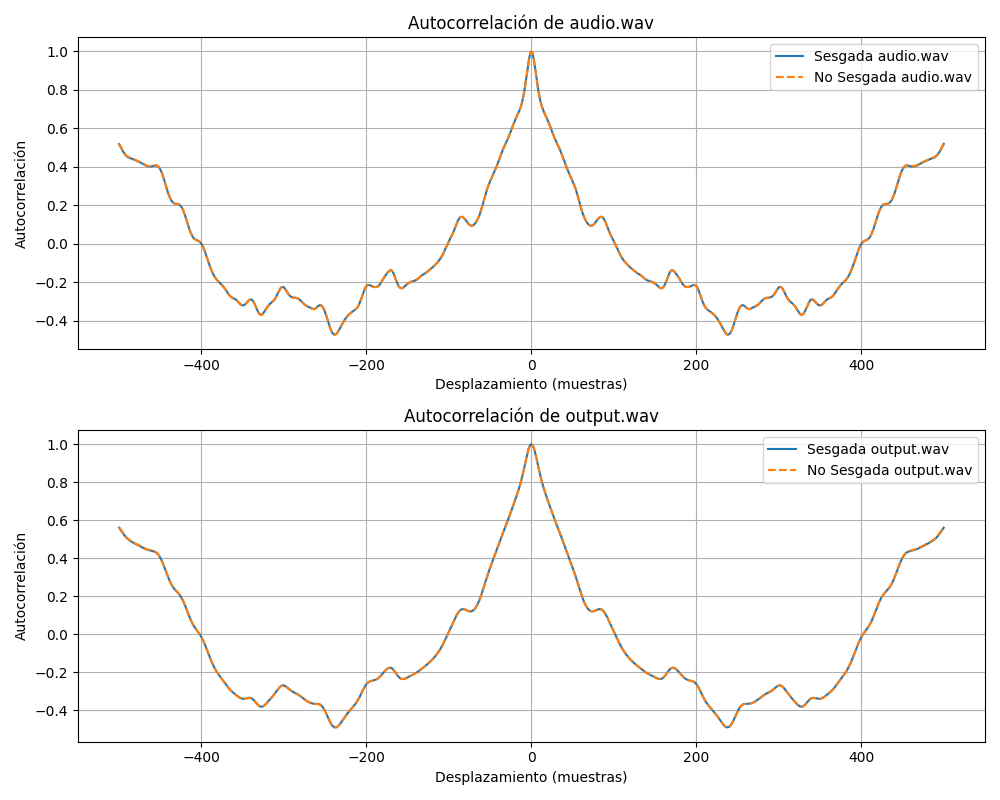
\includegraphics[width=0.7\textwidth]{data/autocorrelacion_sesgada_vs_nosesgada.png}
  \caption{Autocorrelación sesgada y no sesgada de las señales de entrada y salida.}
\end{figure}

\begin{figure}[H]
  \centering
  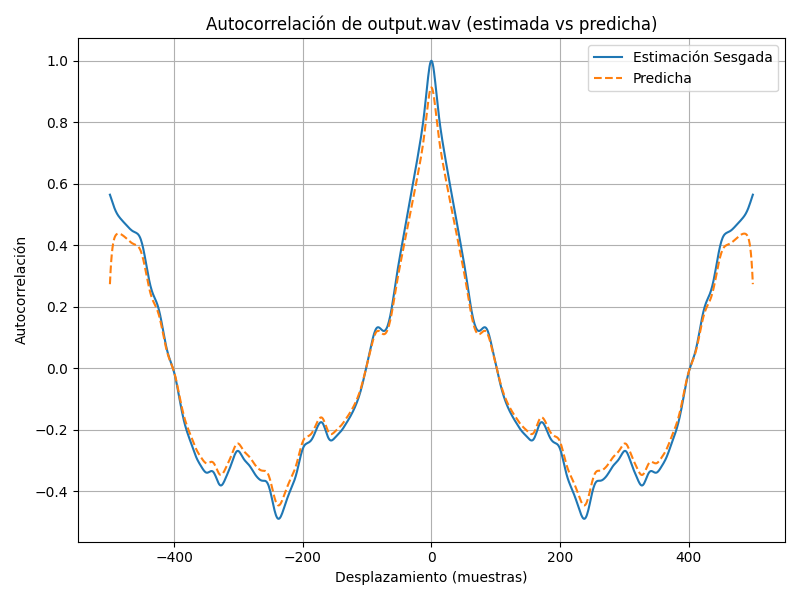
\includegraphics[width=0.7\textwidth]{data/autocorrelacion_predicha.png}
  \caption{Comparación entre autocorrelación estimada y predicha de la señal de salida.}
\end{figure}

% ==== Problema 3 ====
\section*{Problema 3}

Se calcula la correlación cruzada entrada-salida tanto sesgada como no sesgada.
Luego, se compara con la correlación cruzada predicha:
\[
\hat{r}^{(pred)}_{fg}[l] = h^*[-l] \ast \hat{r}_f[l],
\]
y se obtiene un error relativo igual a $0.1333$.

\lstinputlisting[language=Python, caption={Código para el Problema 3}]{src/p3.py}

\begin{figure}[H]
  \centering
  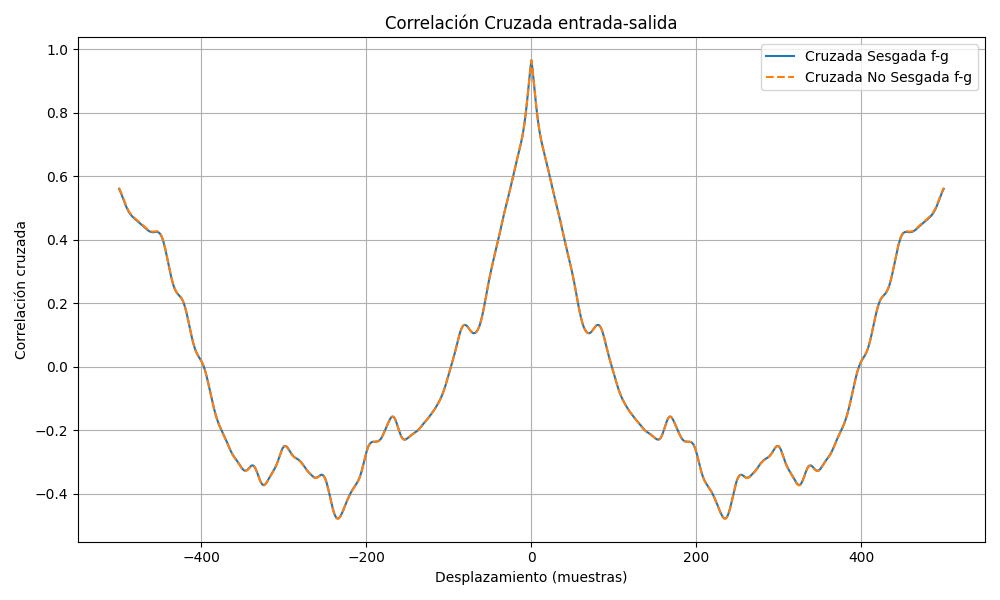
\includegraphics[width=0.7\textwidth]{data/correlacion_cruzada.png}
  \caption{Correlación cruzada sesgada y no sesgada entre entrada y salida.}
\end{figure}

\begin{figure}[H]
  \centering
  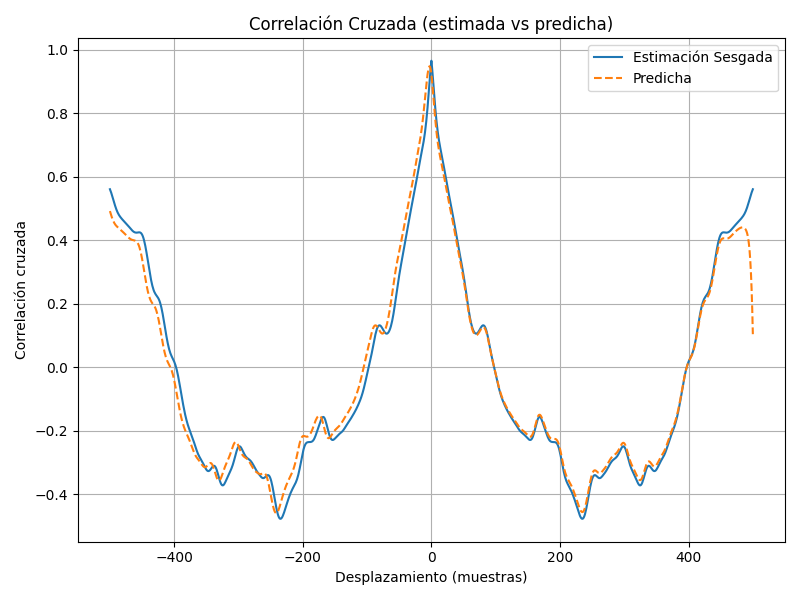
\includegraphics[width=0.7\textwidth]{data/correlacion_cruzada_predicha.png}
  \caption{Comparación entre correlación cruzada estimada y predicha.}
\end{figure}

\section*{Problema 4}

\subsection*{Parte a}

El filtro \texttt{h[n]} es un filtro IIR causal de tipo exponencial. Actua como un filtro pasa bajos, por lo que suaviza la señal de entrada. En un audio se traduce en una reducción del ruido de alta frecuencia, pero también puede causar una pérdida de detalles en la señal. El parámetro $\alpha$ controla la rapidez con la que el filtro atenúa las frecuencias altas: valores cercanos a 1 resultan en una mayor atenuación, mientras que valores cercanos a 0 permiten pasar más frecuencias altas.

El efecto del filtro en $r_g[l]$ y $r_{fg}[l]$ es que ambos se ven suavizados y atenuados en comparación con $r_f[l]$. Esto se debe a que la convolución con el filtro introduce una dependencia temporal, lo que reduce la variabilidad de la señal y, por ende, sus correlaciones.

\subsection*{Parte b}

El efecto de $L_h$ en las estimaciones de autocorrelación y correlación cruzada es que un $L_h$ más grande permite capturar más del efecto del filtro en la señal. Sin embargo, a partir de cierto valor, aumentar $L_h$ tiene un impacto mínimo, ya que los valores de $h[n]$ se vuelven muy pequeños y contribuyen poco a la convolución.

Ahora bien, $L$ determina la ventana de retardos para los cuales se calcula la autocorrelación y correlación cruzada. Un $L$ más grande permite observar más detalles en las correlaciones a largo plazo, pero también más tiempo de cómputo y posible ruido en las estimaciones.

\end{document}
